\documentclass[12pt]{article}

\usepackage{graphicx}
\usepackage{amsmath}
\usepackage[margin=1in]{geometry}
\usepackage{fancyhdr}
\usepackage{enumerate}
\usepackage[shortlabels]{enumitem}
\usepackage[spanish]{babel}
\usepackage{xurl}
\usepackage{tcolorbox}
\usepackage{titlesec}
\usepackage{listings}
\usepackage{xcolor}
\usepackage{pgfplots}
\usepackage{tikz}
\usepackage{cancel}

\titleclass{\subsubsubsection}{straight}[\subsection]

\newcounter{subsubsubsection}[subsubsection]
\renewcommand\thesubsubsubsection{\thesubsubsection.\arabic{subsubsubsection}}
\renewcommand\theparagraph{\thesubsubsubsection.\arabic{paragraph}} % optional; useful if paragraphs are to be numbered

\titleformat{\subsubsubsection}
{\normalfont\normalsize\bfseries}{\thesubsubsubsection}{1em}{}
\titlespacing*{\subsubsubsection}
{0pt}{3.25ex plus 1ex minus .2ex}{1.5ex plus .2ex}

\makeatletter
\renewcommand\paragraph{\@startsection{paragraph}{5}{\z@}%
  {3.25ex \@plus1ex \@minus.2ex}%
  {-1em}%
  {\normalfont\normalsize\bfseries}}
\renewcommand\subparagraph{\@startsection{subparagraph}{6}{\parindent}%
  {3.25ex \@plus1ex \@minus .2ex}%
  {-1em}%
  {\normalfont\normalsize\bfseries}}
\def\toclevel@subsubsubsection{4}
\def\toclevel@paragraph{5}
% \def\toclevel@paragraph{6}
\def\toclevel@subparagraph{6}
\def\l@subsubsubsection{\@dottedtocline{4}{7em}{4em}}
\def\l@paragraph{\@dottedtocline{5}{10em}{5em}}
\def\l@subparagraph{\@dottedtocline{6}{14em}{6em}}
\makeatother

\setcounter{secnumdepth}{4}
\setcounter{tocdepth}{4}

% Set up headers and footers
\pagestyle{fancy}
\fancyhf{}  % Clear previous settings

\fancyhead[L]{Alvarado Ludwig - Vera Julián}
\fancyhead[C]{Simulación Estocástica}
\fancyhead[R]{9 de Marzo de 2025}

\fancyfoot[C]{\thepage}
\fancyfoot[C]{\footnotesize Este trabajo está bajo una licencia CC 4.0. Más info: \url{https://creativecommons.org/licenses/by/4.0/}}

\renewcommand{\headrulewidth}{0.2pt}


% Define R Style for listings
\lstdefinestyle{RStyle}{
  language=R,
  basicstyle=\ttfamily\small,
  keywordstyle=\color{blue}\bfseries,
  commentstyle=\color{green!40!black}\itshape,
  stringstyle=\color{red!70!black},
  numbers=left,
  numberstyle=\tiny\color{gray},
  stepnumber=1,
  numbersep=5pt,
  backgroundcolor=\color{gray!10},
  showstringspaces=false,
  breaklines=true,
  frame=single,
  rulecolor=\color{black},
  captionpos=b,
  morekeywords={generator}
}

% Set RStyle as default
\lstset{style=RStyle}

\begin{document}




\section{\textit{Events and probability}}
\subsection{Punto a}
\subsubsection{Solución}

Se considera una caja con tres canicas de colores rojo, verde y ayuzal como la de la figura \ref{fig:caja-canica}, nos dicen que en el experimento se toma una canica y despues se vuelve a poner en la caja, es decir, si definimos los eventos como:

\begin{itemize}
  \item \(A\) sacar canica verde.
  \item \(B\) sacar canica azul.
  \item \(C\) sacar canica roja.
\end{itemize}

Se afirma que los eventos \(A, B\) y \(C\) son independientes los unos de los otros, ya que, estos no dependen del otro.

\begin{itemize}
  \item \textbf{Espacio muestral (\(\Omega\)):} de acuerdo a la definición ``Es el conjunto de todos los posibles resultados de un experimento aleatorio.'' En este experimento solo se pueden tener diferentes pares de resultados Por lo tanto, la combinación de estos resultados da como resultado el siguiente conjunto:
        \[
        \Omega = \{ (A,A), (A, B), (A, C), (B, A), (B, B), (B, C), (C, A), (C, B), (C, C)  \}
        \]
        Al sacar \(|\Omega|\) este resultado es de \(9\) posibles resultados del experimento. 
  \item \textbf{Probabilidad de cada canica:} el enunciado nos dice que cada canica tiene el mismo chance de ser seleccionada, es decir, una entre tres canicas, por lo tanto, las probabilidades de cada evento se definen como:
        \[
        P(A) = \frac{1}{3} = 0.33\overline{333} \qquad P(B) = \frac{1}{3} = 0.33\overline{333} \qquad P(C) = \frac{1}{3} = 0.33\overline{333}
        \]
        Las dos sacadas son independientes, por lo tanto, se puede aplicar que para cada par \((X, Y)\) se cumpla:
        \[
        P(X) \times P(Y) = \frac{1}{3} \times \frac{1}{3} = \frac{1}{9} = 0.11\overline{111}
        \]
        Por lo tanto, cada punto en el espacio muestral es de \(\frac{1}{9}\).
\end{itemize}



\begin{figure}[ht]
  \centering
  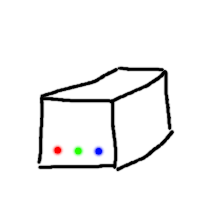
\includegraphics[width=0.4\textwidth]{img/Caja.png}
  \caption{\label{fig:caja-canica} Caja con 3 canicas de colores rojo, verde y azul. Ilustración de los autores elaborada en el software GIMP.}
\end{figure}


\subsection{Punto b}
\subsubsection{Solución}

En este punto nos plantean la misma situación anterior pero los eventos son \textbf{dependientes}, ya que, se saca la primera canica y no se vuelve a meter, es decir, si saco la canica azul como se ve en la figura \ref{fig:caja-2} para la segunda sacada de canica la probabilidad no va a ser la misma, puesto que, hay únicamente dos canicas a sacar. 

\begin{figure}[ht]
  \centering
  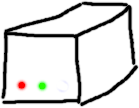
\includegraphics[width=.3\textwidth]{img/Caja2.png}
  \caption{\label{fig:caja-2} Caja con canicas verde y roja. Ilustración de los autores elaborada en el software GIMP.}
\end{figure}


Entonces, el conjunto del espacio muestral \(\Omega\) queda como:

\[
  \Omega = \{ (A, B), (A, C), (B, A), (B, C), (C, A), (C, B)\}
\]

La cardinalidad entonces del conjunto \(\Omega\) es de 6.

Teniendo en cuenta la probabilidad para dos eventos dependientes:

\[
  P(X \cap Y) = P(X|Y) P(Y)
\]

Si sacamos una canica de color rojo (\(P(C)\)) su probabilidad se mantiene como la del mundo anterior \(\frac{1}{3}\). Podemos deducir que en el espacio muestral quedan las canicas azul y verde, si deseamos sacar la azul \((P(B)\), esta está condicionada por el evento anterior de sacar la roja. Teniendo en cuenta, lo anterior, la probabilidad de sacar una canica azul será \(P(B|C) = \frac{1}{2}\). Por lo tanto, al realizar la operación:

\[
  P(B|C)P(C) = \frac{1}{2} \times \frac{1}{3} = \frac{1}{6} = 0.166\overline{666}
\]

Generalizando con \((X, Y)\) siendo un par del espacio muestral \(\Omega\):

\[
  P(X \cap Y) = P(X|Y)P(Y) = \frac{1}{2} \times \frac{1}{3} = \frac{1}{6} =  0.166\overline{666}
\]

En conclusión, la probabilidad para cada canica dado que se saque una antes y no se vuelva a introducir es de \(0.166\overline{666}\). 

\section{\textit{Congruential generators}}
\subsubsection{Solución}

La solución a este ejercicio se puede ver a más profundidad en el archivo \textsf{R} \textit{markdown} adjunto.  

Teniendo en cuenta el siguiente generador:

\[
  X_{n} = (9X_{n-1} + 3) \mod 11
\]

Se utiliza la siguiente función \lstinline|generator()| programada en \textsf{R}.

\begin{lstlisting}
generator <- function(x_n1, n){
  for (i in 1:n){
    print(x_n1)
    x_n1 <- (9 * x_n1 + 3) %% 11
  }
}
\end{lstlisting}

Los \textit{seeds} o semillas ($X_{n-1}$) que sirven para generar todos los ciclos son:

\begin{itemize}
  \item $X_{n-1} = 1:$ Se obtiene la siguiente secuencia $\{1, 1, \cdots \}$, un conjunto de solo unos.
  \item $X_{n-1} = 2:$ Se obtiene $\{2, 10, 5, 4, 6, 2, 10, \cdots \}$.
  \item $X_{n-1} = 3:$ El conjunto es $\{3, 8, 9, 7, 0, 3, 8, \cdots \} $.
\end{itemize}

Al llamar las funciones con estas semillas, se obtiene:

\begin{itemize}
  \item $X_{n-1} = 1:$
\begin{lstlisting}
generator(1, 8)
## [1] 1
## [1] 1
## [1] 1
## [1] 1
## [1] 1
## [1] 1
## [1] 1
## [1] 1
\end{lstlisting}
  \item $X_{n-1} = 2:$
\begin{lstlisting}
generator(2, 8)
## [1] 2
## [1] 10
## [1] 5
## [1] 4
## [1] 6
## [1] 2
## [1] 10
## [1] 5
\end{lstlisting}
  \item $X_{n-1} = 3:$
\begin{lstlisting}
generator(3, 8)
## [1] 3
## [1] 8
## [1] 9
## [1] 7
## [1] 0
## [1] 3
## [1] 8
## [1] 9
\end{lstlisting}
\end{itemize}

Al prestar atención, se puede ver que están todos los números naturales (adoptando el criterio de que el 0 es natural) menores a 11. Ya después, cualquier semilla que se tome hace volver a alguna de esas tres secuencias.



\section{\textit{Uniformity and independence of the unif}}

\subsubsection{Solución}


El siguiente código genera números pseudoaleatorios y se representan gráficamente por medio de un histograma, gráfico de dispersión y un gráfico de autocorrelación para los números pseudoaleatorios generados.

\begin{lstlisting}
    > Nsim = 10^4 # Cantidad de numeros pseudoaleatorios a generar (10,000)
    
    > x=runif(Nsim) # Se almacenan los 10,000 numeros pseudoaleatorios en la variable x 
    
    > x1=x[-Nsim] # Se remueve el ultimo elemento de x (ultimo numero pseudoaleatorio)
                  # y se almacena el restante en la variable x1
                  
    > x2=x[-1] # Se remueve el primer elemento de x (primer numero pseudoaleatorio)
               # y se almacena el restante en la variable x2
               
    > par(mfrow=c(1,3)) # Se ajusta para que las tres graficas queden una 
                        # al lado de la otra en una sola fila

    > hist(x) # Se genera un histograma a partir de x

    > plot(x1, x2) # Se genera un grafico de dispersion entre las variables x1 y x2

    > acf(x) # Se genera un grafico de dispersion para evaluar la autocorrelacion 
             # entre los valores
\end{lstlisting}


Para el diagrama de dispersión, se utilizaron dos variables \textit{x1} que contenía los mismos números pseudoaleatorios generados anteriormente pero sin el último elemento, y lo mismo para la variable \textit{x2}, pero en este caso se removió el primer elemento.

\textbf{¿Por qué se eliminaron algunos elementos para estas variables?}

La razón por la que se hizo esto fue para que en el momento de graficar el gráfico de dispersión estos números pseudoaleatorios estuvieran ordenados de a parejas diferentes, ya que si se dejan los mismos valores para las dos variables, en el gráfico de dispersión estarían sobrepuestos una sobre la otra y se mostraría una línea diagonal, lo cual no es ideal para un gráfico de estos.


\section{\textit{Inverse method for a discrete r.v.}}

Consider the discrete random variable (r.v.) $X$ with probability mass function (\textit{pmf}) given by:

\[
P (X = -1) = 0.2, \quad P (X = 0) = 0.5, \quad P (X = 1) = 0.3
\]





\subsection{Punto a}

Calculate and plot the Cumulative Distribution Function (\textit{CDF}) $F_{X} (x)$ of $X$.
\subsubsection{Solución}

Teniendo en cuenta que la variable aleatoria discreta \textbf{X} toma diferentes valores, para calcular la función de distribución acumulada debemos acumular las probabilidades.
\\
\\
Se tiene:

\begin{align*} 
X &= -1\ \text{ con }\ P(X=-1)=0.2 \\ 
X &= 0\ \text{ con }\ P(X=0)=0.5 \\
X &= 1\ \text{ con }\ P(X=1)=0.3 \\
\end{align*}


Ahora la función de distribución acumulada se construye acumulando las probabilidades:

\begin{itemize}
    \item Para $x < -1: F_X(x) = 0$
    \item Para $-1 \leq x \leq 0: F_X(x) = 0.2$
    \item Para $0 \leq x \leq 1: F_X(x) = 0.2 + 0.5 = 0.7$
    \item Para $x \geq 1: F_X(x) = 0.2 + 0.5 + 0.3 = 1$
\end{itemize}



\begin{lstlisting}
> x <- c(-1, 0, 1) # Valores de la variable aleatoria X
> p <- c(0.2, 0.5, 0.3) # Probabilidad para cada valor de X

> cdf <- cumsum(p) # Se calcula las probabilidades acumuladas con la funcion 'cumsum()'

> f_x <- stepfun(x, c(0, cdf)) # Se inicializa la funcion de distribucion acumulada con la funcion 'stepfun()'

> plot(f_x, xlin=c(-2, 2), main="CDF", xlab="x", ylab=expression(F[X](x)), do.points=TRUE, verticals=TRUE) # Se grafica la funcion de distribucion acumulada
\end{lstlisting}


\textbf{Output}

\begin{figure}[h]
    \centering
    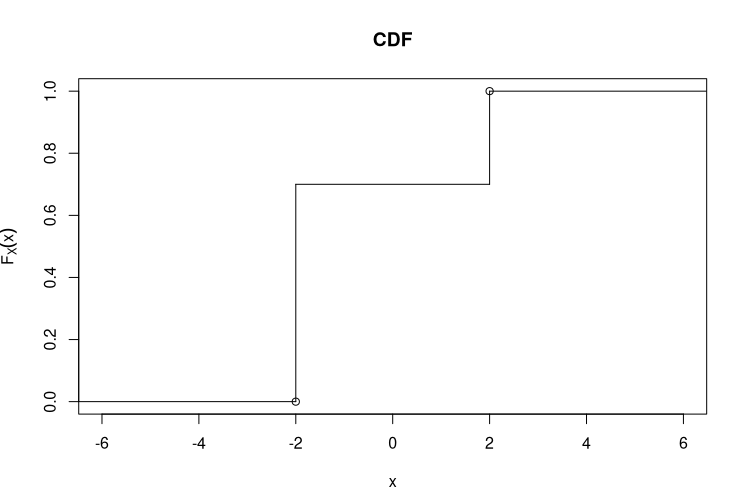
\includegraphics[scale=0.5]{img/cdf.png}
\end{figure}



\subsection{Punto b}

Calculate the expectation $E[X]$ and variance $Var(X)$ of $X$.

\subsubsection{Solución}


Para calcular la esperanza $E[X]$ se multiplica cada valor por su probabilidad y sumando los resultados:
\[E[X] = (-1)(0.2)+(0)(0.5)+(1)(0.3) = 0.1\]

Para calcular la varianza, se necesita primero $E[X^2]$, entonces:
\[E[X^2] = (-1)^2(0.2)+(0)^2(0.5)+(1)^2(0.3) = 0.5\]

Teniendo $E[X^2]$, se puede calcular la varianza:
\[Var(X) = E[X^2] - (E[X])^2 = 0.5-(0.1)^2=0.49\]
La esperanza $E[X]$ es de $0.1$ y la varianza $Var[X]$ es de $0.49$.\newline 




\subsection{Punto c}

Write a program to generate n values of this random variable using the inverse method i.e. by generating random numbers uniformly distributed in (0, 1).

\subsubsection{Solución}


\begin{lstlisting}
n <- 1000 # Tamano de la muestra
u <- runif(n) # Se generan 'n' numeros aleatorios
x <- ifelse(u < 0.2, -1, ifelse(u < 0.7, 0, 1)) # Se establecen las condiciones de la funcion de distribucion acumulada, con respecto a los valores y sus probabilidades

prob <- table(x)/n # Se calculan las probabilidades para cada valor simulado de x

print(prob_empiricas)
\end{lstlisting}


\textbf{Output}


\begin{figure}[h]
    \centering
    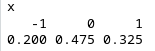
\includegraphics[scale=0.5]{img/table_x.png}
\end{figure}

En este caso, el $20\%$ de las simulaciones dieron como resultado $-1$, el $47.5\%$ dieron como resultado 0 y el $32.5\%$ dieron como resultado 1.



\subsection{Punto d}

Let $n = 100$, run the program, and determine: (i) the aritmetic mean $\bar{X}$ of the simulated values and (ii) the sample standard deviation $S$ of these values. Compare these statistics with the quantities:

\subsubsection{Solución}

Para $n=100$


\begin{lstlisting}
n <- 100 
u <- runif(n)
x <- ifelse(u < 0.2, -1, ifelse(u < 0.7, 0, 1)) 
x_barra <- mean(x) # Se calcula la media muestral
s <- sd(x) # Se calcula la Desviacion estandar muestral

# Resultados
cat("Media muestral =",x_barra, "\n")
cat("Desviacion estandar muestral (s) =",s, "\n")

E_X <- 0.1 # Valor del E[X]
APE1 <- abs(E_X - x_barra)/E_X * 100
cat("Error porcentual absoluto para E[X] =", APE1, "%\n")

SD_X <- 0.7
APE2 <- abs(SD_X - s)/SD_X * 100
cat("Error porcentual absoluto para sqrt(Var(X)) =", APE2, "%\n")
\end{lstlisting}

\textbf{Output}

\begin{lstlisting}
Media muestral = 0.07
Desviacion estandar muestral (s) = 0.7282884
Error porcentual absoluto para E[X] = 30 %
Error porcentual absoluto para sqrt(Var(X)) = 4.041205 %
\end{lstlisting}



\subsection{Punto e}
Repeat d ) with n = 1000.

\subsubsection{Solución}

Para $n=1000$


\textbf{Output}


\begin{lstlisting}
Media muestral = 0.044
Desviacion estandar muestral (s) = 0.6975318
Error porcentual absoluto para E[X] = 56 %
Error porcentual absoluto para sqrt(Var(X)) = 0.3526063 %
\end{lstlisting}




\subsection{Punto f}
Repeat d ) with n = 10000.

\subsubsection{Solución}

Para $n=10000$


\textbf{Output}


\begin{lstlisting}
Media muestral = 0.0845
Desviacion estandar muestral (s) = 0.7064062
Error porcentual absoluto para E[X] = 15.5 %
Error porcentual absoluto para sqrt(Var(X)) = 0.9151645 %
\end{lstlisting}

Podemos concluir que al aumentar el tamaño de la muestra $n$, las estimaciones se aproximan cada vez más a los valores teóricos esperados.




\section{\textit{Inverse method for a continuos r.v}}

Consider the continuos random variable $X$ with probability density function (\textit{pdf}) given by:

\[
f_{X} (x) =
\begin{cases}
  3(x - 1)^{2} \quad \text{for} \quad 1 < x \leq 2, \\
  0 \quad \text{otherwise}
\end{cases}
\]


\subsection{Punto a}

Find the following probabilities: (i) $P(X \leq 1)$, (ii) $P(1 < X \leq 1.5)$, (iii) $P(X \geq 1.5)$

\subsubsection{Solución}

Se debe hacer uso de la integral para poder hacer dichas probabilidades, se puede obtener la función $f_{X}(x)$ y graficarla tal como:

\begin{center}
    \begin{tikzpicture}
        \begin{axis}[
            axis x line=middle,
            axis y line=middle,
            xlabel={$x$},
            ylabel={$f_X(x)$},
            samples=100,
            domain=0:3,
            ymin=0, ymax=3,
            xmin=0, xmax=3,
            xtick={1,2},
            ytick={1,2},
            enlargelimits=true,
            clip=false
        ]
        % Plot the function for 1 < x <= 2
        \addplot[
            domain=1:2,
            thick,
            blue
        ] {3*(x-1)^2} node[pos=0.8, above] {};
        
        % Add zero function elsewhere
        \addplot[
            domain=0:1,
            thick,
            blue
        ] {0};
        \addplot[
            domain=2:3,
            thick,
            blue
        ] {0};

        % Add open circle at (1,0) and closed circle at (2,3)
        \fill[white,draw=blue] (axis cs:1,0) circle (2pt); % Open dot
        \fill[blue] (axis cs:2,3) circle (2pt); % Closed dot

        \node at (axis cs:2.2,2) {\small $f_X(x) = 3(x-1)^2$};
    \end{axis}
    \end{tikzpicture}
\end{center}

Ahora, se obtienen las probabilidades:

\begin{itemize}
  \item $P(X \leq 1):$

        Para valores menores a 1 el valor de $f_{X}(x)$ es constante igual a 0, por lo tanto, al hacer la siguiente integral:
        \[
        P(X\leq 1) = \int_{-\infty}^{1} f_{X}(x) dx
        \]
        Reemplazando $f_{X}(x)$ con la \textit{pdf} se tiene que:
        \[  
        P(X\leq 1) = \int_{-\infty}^{1} 0 dx = 0
        \]
        Por lo tanto, $P(X\leq 1) = 0 $, o en palabras, la probabilidad de que la variable aleatoria $X$ sea menor o igual a 1 es de 0.
  \item $P(1 < X \leq 1.5):$

        Siguiendo el mismo proceso del punto anterior, pero ahora se va a integral sobre el intervalo $[1, 1.5]$, por lo tanto:
        \[
        P(1 < X \leq 1.5) = \int_{-\infty}^{1} 3(x-1)^{2} dx
        \]
        Esta integral definida es bastante sencilla de resolver, sin embargo, para ahorrar tiempo y espacio se va a usar ayuda del software \textit{Geogebra} para resolver las integrales, por lo tanto, con el comando \lstinline|Integral(3(x-1)^{2},1,1.5)| se obtiene $P(1 < X \leq 1.5) = 0.125$, entonces, la probabilidad de que la variable $X$ esté entre $1$ y $1.5$ es de $0.125$.
  \item $P(X \geq 1.5):$

        El intervalo correcto en este caso sería $[1.5, \infty]$, sin embargo, a partir de $x > 2$ la función es 0, por lo tanto, se va a tomar el intervalo de $[1.5, 2]$.
        \[
        P(X \geq 1.5) = \int_{1.5}^{2} 3(x-1)^{2} dx
        \]
        Utilizando en \textit{Geogebra} \lstinline|Integral(3(x-1)^{2},1.5,2)| se obtiene un resultado de $P(1.5 < X \leq 2) = 0.875$, es decir, la probabilidad de que la variable aleatoria $X$ esté entre 1.5 y 2 es bastante alta, mientras que para mayor a 2 esta es 0.
\end{itemize}



\subsection{Punto b}
\subsubsection{Solución}

Recordando que para calcular el valor esperado $E$ de $X$ se debe realizar la integral:

\[
  E[X] = \int_{-\infty}^{\infty} x f(x) dx
\]

Teniendo en cuenta la \textit{pdf} el intervalo por el que se va a integrar es $[1, 2]$. En este caso, la integral sí se va a realizar de manera manual con el fin de expandir más el punto, sin embargo, al final se va a realizar la comprobación mediante \textit{Geogebra}. Definiendo el valor esperado $E$ como la siguiente integral:

\[
E[X] = \int_{1}^{2} x \times 3(x - 1)^{2} dx
\]

Se puede sacar el término constante 3 afuera de la integral, resolver el binomio y multiplicar el término $x$ para quedar de la siguiente manera:

\begin{align*}
  E[X] &= 3 \int_{1}^{2} x(x^{2} - 2x + 1) dx \\
       &= 3 \int_{1}^{2} (x^{3} - 2x^{2} + x) dx 
\end{align*}

Tomando en cuenta la propiedad de linealidad de la integral se tiene:

\[
  \int_{1}^{2} x^{3} dx = \frac{x^{4}}{4}, \quad \int x^{2} dx = \frac{x^{3}}{3} , \quad \int xdx = \frac{x^{2}}{2}  
\]

Haciendo cada integral sobre el intervalo, se tiene:
\begin{align*}
  \left[\frac{x^{5}}{5} \right]_{1}^{2} &= \frac{32}{5} - \frac{1}{5} = \frac{31}{5} \\
  \left[\frac{x^{4}}{4} \right]_{1}^{2} &= \frac{16}{4} - \frac{1}{4} = \frac{15}{4}\\
  \left[\frac{x^{3}}{3} \right]_{1}^{2} &= \frac{8}{3} - \frac{1}{3} = \frac{7}{3}
\end{align*}

Ahora, se puede volver a donde se estaba para calcular el valor esperado reemplazando con los valores obtenidos de las integrales:

\begin{align*}
  E[X] &= 3 \left( \frac{15}{4} - 2 \times \frac{7}{3} + \frac{3}{2} \right) \\
       &= 3 \left( \frac{15}{4} - \frac{14}{3} + \frac{3}{2} \right) \\
       &= 3 \times \frac{7}{12} = \frac{21}{12} = \frac{7}{4} \\
  E[X] &= 1.75
\end{align*}

Por lo tanto, el valor esperado $E$ de $X$ es $1.75$. Al utilizar la función de \textit{Geogebra} \lstinline|Integral(x * (3(x-1)^{2}),1,2)| se obtiene el mismo resultado de $1.75$

Teniendo en cuenta las definiciones presentadas en el PDF \textit{Introducción a probabilidad} de Carlos Ricardo Bojacá encontradas en el AVATA del presente curso, se toma:

Valor esperado o media ($\mu$)en variable continua:

\[
\mu = E(X) = \int_{-\infty}^{\infty} x \times f(x) dx
\]

Varianza:

\[
\sigma^{2} = V(X) = E(X - \mu)^{2} = E(X^{2}) - \mu^{2}
\]

Sabemos que la media $\mu$ es lo mismo que el valor esperado al cuadrado, entonces, calcuando $E[X^{2}]$:

\begin{align*}
  E[X^{2}] &= \int_{1}^{2} x^{2} f_{X} (x) dx \\
  E[X^{2}] &= 3 \int_{1}^{2} x^{2} (x-1)^{2} dx
\end{align*}

Debido a que el procedimiento manual se hizo con el valor esperado, vamos a saltar utilizando el comando de \textit{Geogebra} \lstinline|Integral(x^2 * (3(x-1)^{2}),1.5,2)|, dando un valor de $E[X^{2}] = 3.1$, ahora para hallar $\mu^{2}$

\[
\mu^{2} = E[X]^{2} = 1.75^{2} = 3.0625
\]

Entonces, la varianza $\mathrm{Var}(X)$:

\begin{align*}
  \mathrm{Var} &= E[X^{2}] - E[X]^{2} \\
               &= 3.1 - 3.0625 \\
               &= 0.0375
\end{align*}

En conclusión, el valor esperado es de $E[X] = 1.75$ y la varianza de $\mathrm{Var}(X) = 0.0375$, los datos varían muy poco de la media.

\subsection{Punto c}

Find the CDF $F_{X}(x)$ of $X$. Plot this function

\subsubsection{Solución}

Se sabe por definición que la \textit{cdf} (\textit{Continuos Random Variable}) es encontrada integrando la \textit{pdf}:

\[
F(X) = \int_{-\infty}^{x} f(t) dt
\]

Se va a encontrar $F(x)$ integrando $f(x)$ sobre los diferentes intervalos:

\begin{align*}
  \text{para } 1 < x \leq 2 : \quad F(x) &= \int_{1}^{x} 3(t-1)^{2} dt \\ 
                                         &= \int_{1}^{x} (3t^{2} - 6t + 3) dt \\ 
                                        I&= [t^{3} - 3t^{2} + 3t]_{1}^{x} \\ 
                                         &= (x^{3} - 3x^{2} + 3x) - (1^{3} - 3(1^{2}) + 3(1)) \\ 
                                         &= x^{3} - 3x^{2} + 3x - 1 \\
  \text{para otro caso: } \quad F(x) &= \int_{-\infty}^{x} 0 dt = 0 
\end{align*}

Al poner ambos juntos, se escribe $F$ como:


\[
F (x) =
\begin{cases}
  x^{3} - 3x^{2} + 3x - 1, \quad \text{para} \quad 1 < x \leq 2 \\
  0, \qquad \text{de otra manera}
\end{cases}
\]

Ahora, para su gráfica usando el paquete \texttt{pgfplots} de \LaTeX:

\begin{center}

\begin{tikzpicture}
    \begin{axis}[
        axis lines = middle,
        xlabel = {$x$},
        ylabel = {$F(x)$},
        samples = 100,
        domain = 0:3,
        ymin = -2, ymax = 2,
        xmin = 0, xmax = 3,
        xtick = {1,2},
        ytick = {-1,0,1},
        clip=false
    ]
        % Define the piecewise function
        \addplot[domain=1:2, thick, blue] {x^3 - 3*x^2 + 3*x - 1};
        \addplot[domain=0:1, thick, red] {0};
        \addplot[domain=2:3, thick, red] {0};

        % Open circle at (1,0) to indicate discontinuity
        \draw[fill=white, thick] (axis cs:1,0) circle[radius=2pt];
        % Closed circle at (1,F(1))
        \draw[fill=blue, thick] (axis cs:1,-1) circle[radius=2pt];
        % Closed circle at (2,F(2))
        \draw[fill=blue, thick] (axis cs:2,0) circle[radius=2pt];
    \end{axis}
\end{tikzpicture}
\end{center}

\subsection{Punto d}

Show how to simulate $X$ with this $CDF$ using the inversion method.

\subsubsection{Solución}

Ya se tiene la \textit{cdf} $F(x) = x^{3} - 3x^{2} + 3x - 1, 1 < x \leq 2$, se puede invertir resolviendo para $x$ en la ecuación $F(x) = u$, por lo tanto, al factorizar $F(x)$, se obtiene:

\begin{align*}
  F(x) &= x^{3} - 3x^{2} + 3x - 1 = u\\
     u &= (x-1)^{3} \\
  \sqrt[3]{u} &= \sqrt[\cancel{3}]{(x-1)^{\cancel{3}}} \\
  \sqrt[3]{u} + 1 &= x
\end{align*}

Por lo tanto, la inversa del \textit{cdf} es:

\[
  x = \sqrt[3]{u} + 1
\]

Sea $U \sim U(0, 1)$. Entonces, para simular $X$ con la \textit{cdf} será:

\[
X = \sqrt[3]{U} + 1
\]


\subsection{Punto d}

Write a program in \textsf{R} that draws 1000 samples of $X$. Plot a normalized histogram of the sample along with the \textit{pdf} of $X$.

\subsubsection{Solución}

Debido a que $U$ se distribuye uniformemente sobre 0 y 1, la función \lstinline|runif()| permite hacer esta distribución y computa una simulación 1000 veces y almacena el resultado el resultado en el vector $U$. La variable $X$ es un vector resultado de sacar la raíz cúbica más uno al vector $U$. Por último, se presenta el histograma en la figura \ref{fig:fig1} muestra una mayor frecuencia de $X$ en valores más cercanos a $2.0$, se puede ver un comportamiento exponencial.

\begin{lstlisting}
U = runif(1000)
X = U ^ (1 / 3) + 1
hist(X)
\end{lstlisting}

\begin{figure}[ht]
  \centering
  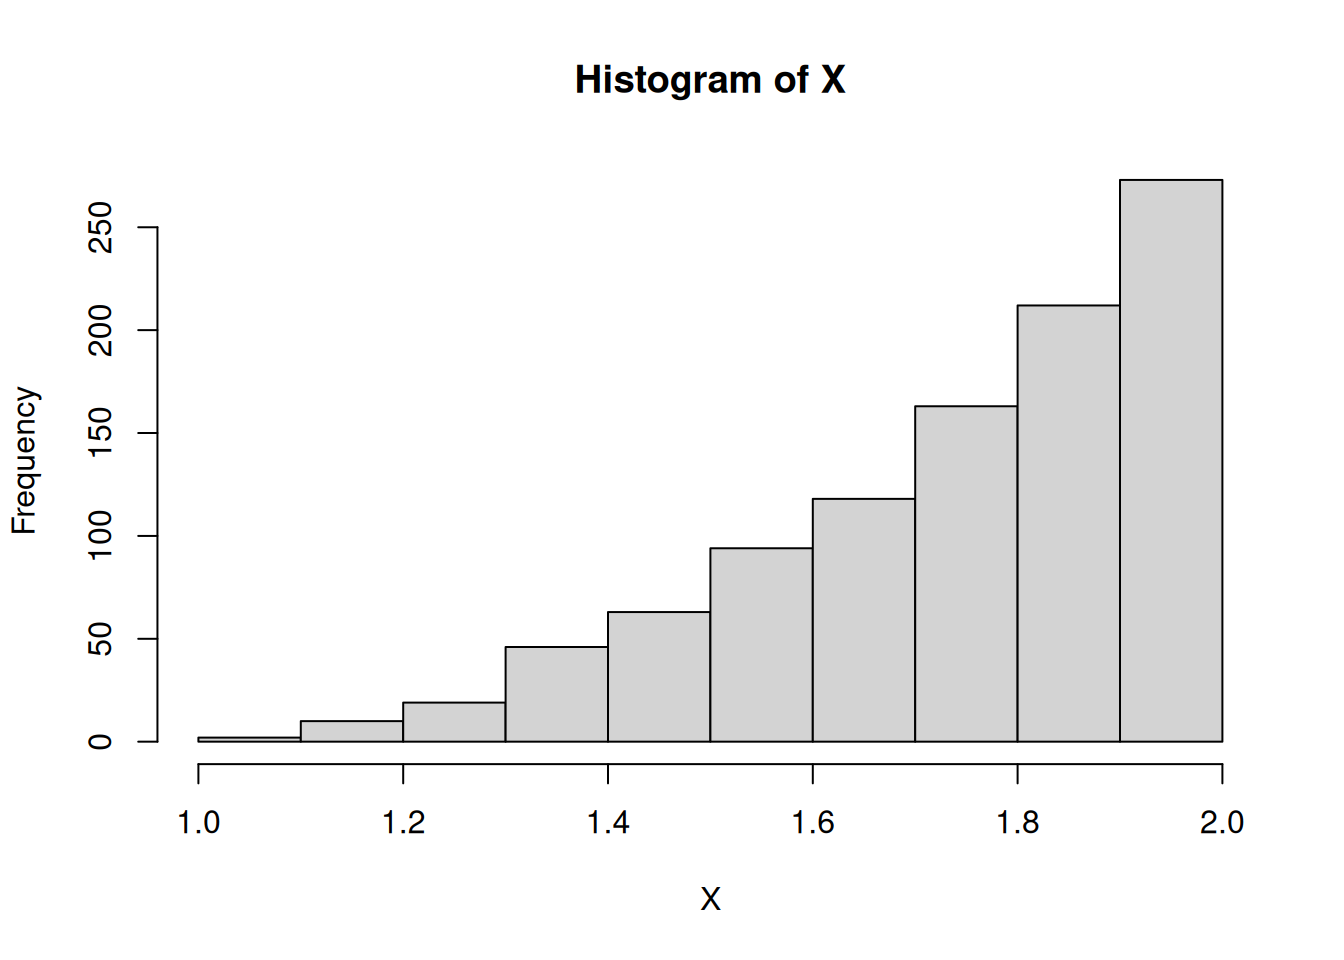
\includegraphics[width=0.5\textwidth]{img/histograma.png}
  \caption{\label{fig:fig1} Histograma de la v.a $X$}
\end{figure}






\section{\textit{Monte Carlo Integration}}

With respect to the following integrals: (i) Find their exact value analytically or with software (e.g., \texttt{WolframAlpha}), (ii) with Monte Carlo integration approximate the integrals and compare with the exact answer.

\subsubsection{Solución}

\subsubsection{$\int_{0}^{1} \exp{e^{x}} dx$}

De acuerdo a \textit{WolframAlpha}, la solución se realiza con la función elemental $\mathrm{Ei(x)}$, según el programa imprime la siguiente solución:

\[
\int_{0}^{1} e^{e^{x}}dx = \mathrm{Ei}(e) - \mathrm{Ei}(1) \approx 6.31656
\]

En el presente trabajo no se busca profundizar acerca de la función elemental utilizada, por lo tanto, se procede a realizar la integración por Monte Carlo para realizar la comparación con el valor arrojado por \textit{WolframAlpha}.

Se toma entonces que el valor esperado $E[g(X)]$ se define como el valor arrojado por WolframAlpha:

\[
E[g(X)] = \frac{\int_{a}^{b}g(x) dx}{b - a} = \frac{6.31656}{1 - 0} = 6.31656 
\]

Según la guía del taller, debemos tomar:

\[
\sum_{i = 1}^{n} \frac{g(X_{i})}{n}
\]

Para así obtener un valor apróximado al valor esperado, el siguiente código en \textsf{R} (para visualizar mejor el resultado visite el \textit{notebook} adjunto a la entrega) muestra el valor estimado del valor de $E[g(x)]$

\begin{lstlisting}
a <- 0
b <- 1
N <- 100000
X <- runif(N, a, b)
g <- function(x) exp(exp(x))
gX <- g(X)
plot(X, gX)
H <- mean(gX)
\end{lstlisting}

Al imprimir el valor de $H$ para esta simulación da un valor de $6.309694$, similar al arrojado por \textit{WolframAlpha}, la diferencia entre ambos resultados es de $0.006866$. Si incrementamos $N$ en la simulación la diferencia va a disminuir y si tiende a infinito, este va a llegar a ser exacto.


\subsubsection{$\int_{-2}^{2} e^{x + x^{2}} dx$}

Se toma el mismo proceso que en el punto anterior. Valor arrojado por \textit{WolframAlpha}:

\[
\int_{-2}^{2} e^{x + x^{2}} dx = \frac{\sqrt{\pi} \left(\mathrm{erfi} \left(\frac{3}{2} \right) + \mathrm{erfi} \left(\frac{5}{2} \right) \right)  }{2 \sqrt[4]{e}} \approx 93.1628
\]

Donde $\mathrm{erfi}$ es la función error.

Para obtener el valor esperado $E[g(x)]$:

\begin{align*}
  E[g(x)] &= \frac{\int_{-2}^{2} e^{x + x^{2}} dx}{b - a}  \\
  &= \frac{93.1628}{2 - (-2)} \approx 23.2907
\end{align*}

Ahora, el código en \textsf{R} para realizar la simulación

\begin{lstlisting}
a <- -2
b <- 2
N <- 10000
X <- runif(N, a, b)
g <- function(x) exp(x + x^2)
gX <- g(X)
plot(X, gX)
(H <- mean(gX))
\end{lstlisting}

Se puede ver en el \textit{notebook} que el valor de $H$ es de $23.16239$, haciendo $E[g(x)] - H$ da una diferencia de $0.12831$, la integración de Monte Carlo muestra valores cercanos.

\subsubsection{$\int_{0}^{\infty} x(1 + x^{2})^{-2} dx$}

Solución \textit{WolframAlpha}:

\[
\int_{0}^{\infty} \frac{x}{(1 + x^{2})^{2}} dx = \frac{1}{2} 
\]

Se puede realizar el siguiente cambio de variable:

\[    
y = \frac{1}{x+1} , dy = - \frac{dx}{(x+1)^{2}} = -y^{2} dx
\]

Entonces, con $h(y) = \frac{g \left( \frac{1}{y} - 1\right) }{y^{2}}$:

\[
\theta = \int_{0}^{1} h(y) dy
\]

Puesto de esta manera, la integral queda como:

\[ 
\int_{0}^{1} \frac{\frac{ \frac{1}{y} - 1 }{ (1 + (\frac{1}{y} - 1)^{2} )^{2}}}{y^{2}} dy
\]

La implementación en \textsf{R} es la siguiente: 


\begin{lstlisting}
a <- 0
b <- 1
N <- 100000 
X <- runif(N, a, b)
g <- function(y) ((1/y - 1)/(1 + (1/y - 1)^2)^2)/y^2
gX <- g(X)
plot(X, gX)
(H <- mean(gX))
\end{lstlisting}

Al imprimir $H$, da un valor de $0.4986839$ (vea el \textit{notebook} adjunto). Siendo un valor muy preciso para el valor real de la integral.



\subsubsection{$\int_{0}^{1} \int_{0}^{2} e^{(x + y)^{2}} dydx$}

Solución de \textit{WolframAlpha}:

\[ 
\int_{0}^{1} \int_{0}^{2} e^{(x + y)^{2}} dydx = \frac{1}{2} (e^{4}(1 - 4F(2)) + e^{9} (6 F(3) - 1) - \sqrt{\pi} \ \mathrm{erfi}(1) - 1 + e  ) \approx 275.884
\]

Donde $\mathrm{erfi}$ es la función error y $F(z)$ es la función de Dawson.

El valor esperado $E[g(X, Y)]$ será:

\[
E[g(X, Y)] = \frac{\int_{0}^{1} \int_{0}^{2} e^{(x + y)^{2}} dydx}{(b_{x} - a_{x}) (b_{y} - a_{y})}
\]

Debido a que estamos ante una integral doble, se utilizan dos v.a $(X, Y)$ y el divisor es la multiplicación de la resta de cada intervalo de integración. Por lo tanto, el valor esperado es:

\[
E[g(X, Y)] = \frac{275.884}{(1 - 0) (2 - 0)} = 137.942
\]

Ahora, el siguiente programa en \textsf{R} permite realizar la aproximación a la integral, sigue la misma dinámica que con los anteriores puntos, pero utilizando dos intervalos de integración y añadiendo otro parámetro para la función $g$

\begin{lstlisting}
ax <- 0
bx <- 1
ay <- 0
by <- 2
N <- 1e5
runifX <- runif(N, ax, bx)
runifY <- runif(N, ay, by)
g <- function(x, y) exp((x + y)^2)
gXY <- g(runifX, runifY)
(H <- mean(gXY))
\end{lstlisting}

Al ejecutarse (mirar el \textit{notebook}), muestra un valor de $136.6747$, una diferencia de 1.2674 con respecto al valor esperado $E[g(X, Y)]$.

En este sexto punto se comprobó que el método de Monte Carlo sirve muy bien para aproximar integrales definidas y al comparar los resultados con el valor exacto, este método se acerca mucho más a medida que $N$ se incrementa, tal como se explicaba en clase y también en la ley de los grandes números.





\section{\textit{Estimating} \(\pi\)}

\subsection{Punto a}
\subsubsection{Solución}

Se tiene en cuenta que las variables \textit{\textbf{X}} y \textit{\textbf{Y}} son independientemente e idénticamente distribuidas, y su distribución uniforme esta en el intervalo $[-0.5, 0.5]$. Con respecto a lo anterior, las probabilidades de que ambas variables estén dentro de los intervalos $[a,b]\ \times\ [c,d]$ es el producto de las probabilidades individuales:


\[P((X,Y) \in [a,b]\times[c,d]) = P(a\leq X \leq b)\ \cdot P(c\leq Y \leq d)\]

Para calcular la probabilidad en un subintervalo donde su distribución es uniforme, se tiene que la probabilidad de que \textit{\textbf{X}} esté en el intervalo $[a,b]$ y \textit{\textbf{Y}} en el intervalo $[c,d]$ seran proporcionales a la longitud del intervalo:

Para \textit{\textbf{X}}:

\[P(a \leq X \leq b) = \frac{longitud\ del\ intervalo}{longitud\ del\ intervalo\  total} = \frac{b-a}{0.5-(-0.5)} = \frac{b-a}{1} = b-a\]

Para \textit{\textbf{Y}}:

\[P(c \leq Y \leq d) = \frac{longitud\ del\ intervalo}{longitud\ del\ intervalo\  total} = \frac{d-c}{0.5-(-0.5)} = \frac{d-c}{1} = d-c\]


Así pues, tendremos que la probabilidad de que \textit{\textbf{X}} y \textit{\textbf{Y}} esté en el intervalo $[a,b] \times [c,d]$ es:

\[P((X,Y) \in [a,b] \times [c,d]) = (b-a) \times (d-c)\]



\subsection{Punto b}


\subsubsection{Solución}

Como \textit{\textbf{X}} y \textit{\textbf{Y}} son variables aleatorias uniformemente distribuidas e independientes, la probabilidad de que un punto \textit{$(X,Y)$} esté dentro de una región \textbf{$A$} dentro del intervalo $[-0.5,0.5] \times [-0.5,0.5]$ dependerá del área que ocupa \textbf{$A$} dentro de este intervalo total.

\[P((X,Y) \in A) = \frac{Area\ de\ A}{Area\ total\ del\ dominio}\]

Dado que el dominio original es $[-0.5, 0.5] \times [-0.5,0.5]$ tiene un área total de:

\[(0.5-(-0.5)) \times (0.5-(-0.5))=1\times1=1\]

Por consiguiente, la probabilidad de que \textit{$(X,Y)$} esté en un subconjunto \textbf{$A$} dentro de este dominio simplemente se reduce a:

\[P((X,Y) \in A) = Area\ de\ A\]


\subsection{Punto c}
\subsubsection{Solución}

Se identifica que la ecuación $x^2+y^2=r^2$ representa un círculo centrado en el origen con un radio \textbf{r}, para este ejercicio en específico $r=0.5$, por lo que la ecuación del círculo queda de la siguiente manera:

\[x^2+y^2=0.5^2=0.25\]

Se debe tener en cuenta que, como se esta trabajando en un cuadrado $[-0.5,0.5] \times [-0.5,0.5]$, el circulo queda totalmente contenido dentro del mismo.


Ahora para calcular el área de $A$, se tiene que:

\[\pi r^2=\pi(0.5)^2=\pi\times0.25=0.25\pi\]

Sin embargo, como el círculo esta completamente contenido dentro del cuadrado el área de $A$ es simplemente el área del círculo completo:

\[Area\ de\ A\ =0.25\pi\]

\[Area\ de\ A\ \approx0.25(3.1416)\approx0.7854\]

Se concluye que la región $A$ es el círculo de radio $0.5$ dentro del cuadrado de lado 1, y su área es de aproximadamente $0.7854$. Esta será la probabilidad de que un punto \textit{$(X,Y)$} generado aleatoriamente dentro del cuadrado pertenezca a $A$.


\subsection{Punto d}
\subsubsection{Solución}

Según la definición de la variable aleatoria $Z$, está tomara el valor de \textbf{1} si el punto $(X,Y)$ está dentro del círculo de radio 0.5 centrado en el origen, y tomará el valor de \textbf{0} si el punto está fuera de ese círculo. 


Para el valor esperado $E[Z]$, como $Z=1$ solo cuando el punto $(X,Y)$ cae dentro del círculo, la probabilidad de que eso ocurra es la proporción del área del círculo respecto al área total del dominio $[-0.5,0.5]\times[-0.5,0.5]$, entonces:

\[E[Z] = \frac{Area\ del\ circulo}{Area\ del\ cuadrado} = \frac{\pi r^2}{(0.5-(-0.5))^2}=\frac{\pi(0.5)^2}{1}=\frac{\pi}{4}\]


Por ende, el valor esperado $E[Z]$ es:

\[E[Z]=\frac{\pi}{4}\]



\subsection{Punto e}
\subsubsection{Solución}

\begin{lstlisting}
> n <- 10000 # Tamano de la muestra
> X <- runif(n, -0.5, 0.5) # Se generan 'n' numeros aleatorios en el intervalo [-0.5,0.5] y se almacenan en la variable X
> Y <- runif(n, -0.5, 0.5) # Se generan 'n' numeros aleatorios en el intervalo [-0.5,0.5] y se almacenan en la variable Y
> Z <- ifelse(X^2+Y^2<=0.5^2,1,0) # Verificar si los puntos caen o no dentro del circulo
> pi_estimado <- 4 * mean(Z) # Se estima pi
> print(paste("Estimacion de pi con", n, "muestras:",pi_estimado)
\end{lstlisting}

\textbf{Output}

\begin{figure}[h]
    \centering
    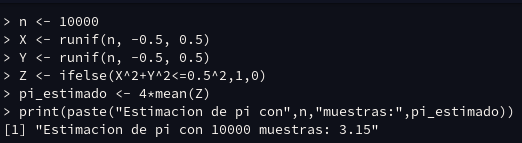
\includegraphics[scale=0.5]{img/output-7.png}
\end{figure}
\end{document}


\section{\textit{Estimating expected values with Monte Carlo}}

For uniform (0, 1) random variables $U_{1}, U_{2}, \dots$ define:

\[
N = \min \left\{n : \sum_{i = 1}^{n} U_{i} > 1 \right\}
\]

That is, $N$ is equal to the number of random numbers that must be summed to exceed 1.


Las simulaciones se realizan creando dos funciones \texttt{N()} y \texttt{En()} que se van a utilizar para las simulaciones de los puntos, el código que se presenta en el \textit{notebook} es

\begin{lstlisting}
N <- function(){
  total <- 0
  count <- 0 
  while (total <= 1){
    total <- total + runif(1, 0, 1)
    count <- count + 1
  }
  return (count)
}

En <- function(N) { 
  samples <- replicate(N, N())
  return (mean(samples))
}
\end{lstlisting}


\subsection{Punto a}

Estimate $E[N]$ by generating 100 values of $N$.

\subsection{Solución}

Llamando la función \texttt{En(100)}, se obtiene un valor estimado de:


\[
 E[100] = 2.72
\]


\subsection{Punto b}

Estimate $E[N]$ by generating 1000 values of $N$.

\subsection{Solución}

Llamando la función \texttt{En(1000)}, se obtiene un valor estimado de:


\[
 E[100] = 2.729
\]





\subsection{Punto c}

Estimate $E[N]$ by generating 10000 values of $N$.

\subsection{Solución}

Llamando la función \texttt{En(10000)}, se obtiene un valor estimado de:


\[
 E[100] = 2.71952
\]



\subsection{Punto d}

What do you think is the value of $E[N]$?

\subsection{Solución}


A medida que el $N$ de la función \texttt{En(N)} va incrementando, este parece acercarse cada vez más al valor de la constante $e$, lo cual, para uno de los autores de este documento, lo hace muy bonito, ya que, este número aparece por todo lado, y descubrir otra manera más de encontrarlo es algo emocionante! 



\end{document}
